\chapter{Teorija}

U ovom poglavlju, nakon uvodnog poglavlja, uobičajeno se detaljnije opisuje
metodologija koja će se primijenti u rješavanju završnog zadatka/diplomskog
rada, itd. Dakle navodi se opis primijenjenog modela, teorije i sl.

\subsection{Opis modela}
Opis modela, teoretskog, matematičkog, eksperimentalnog ili koji je već
primijenjen u radu. Primjerice model razmatran u radu prikazan je relacijom~\eqref{eq:linmodboc1}
\begin{equation}\label{eq:linmodboc1}
\begin{aligned}
  \Delta \dot \beta  &= \frac{{Y_\beta ^0 }}
{{u^0 }}\Delta \beta  + \frac{{Y_p^0 }}
{{u^0 }}\Delta p + \left( { - 1 + \frac{{Y_r^0 }}
{{u^0 }}} \right)\Delta r + \frac{{g\cos \theta ^0 }}
{{u^0 }}\Delta \phi  + \frac{{Y_{\delta _n }^0 }}
{{u^0 }}\Delta \delta _n   \\
  \Delta \dot p &= L_\beta ^0 \Delta \beta  + L_p^0 \Delta p + L_r^0 \Delta r + L_{\delta _\ell  }^0 \Delta \delta _\ell   + L_{\delta _n }^0 \Delta \delta _n   \\
  \Delta \dot r &= N_\beta ^0 \Delta \beta  + N_p^0 \Delta p + N_r^0 \Delta r + N_{\delta _\ell  }^0 \Delta \delta _\ell   + N_{\delta _n }^0 \Delta \delta _n   \\
  \Delta \dot \phi  &= \Delta p + \tan \theta ^0 \Delta r  \\
  \Delta \dot \psi  &= \frac{{\Delta r}}
{{\cos \theta ^0 }} \:, \\ 
\end{aligned} 
\end{equation}
ili u matričnom zapisu
\begin{equation} 
\Delta \mathbf{\dot{X}} = {\mathbf{A}}\Delta {\mathbf{X}} +
{\mathbf{B}\Delta\mathbf{e}}\:,
\end{equation} 
Poželjno je koristiti i slike, kada to može doprinijeti preglednosti i uvidu u model (kao
npr. slika~\ref{fig:bocgib}). 
%
\begin{figure}[!h]
	\centering
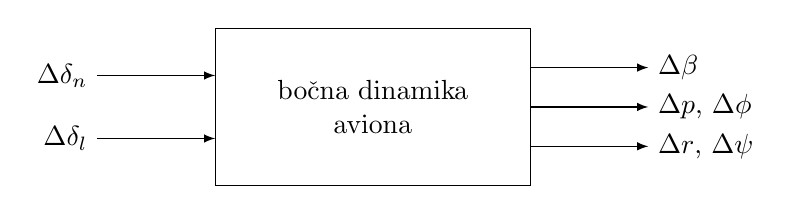
\begin{tikzpicture}
	\draw (0,0) rectangle (4,2);
	\draw (2,1) node[text width=3cm, text badly centered]{bo\v cna dinamika aviona};
	\draw[latex-] (0,0.6)--(-1.5,0.6) node[left] {$\Delta \delta_l$};
	\draw[latex-] (0,1.4)--(-1.5,1.4) node[left] {$\Delta \delta_n$};
	\draw[-latex] (4,0.5)--(5.5,0.5) node[right] {$\Delta r$, $\Delta \psi$};
	\draw[-latex] (4,1)--(5.5,1) node[right] {$\Delta p$, $\Delta \phi$};
	\draw[-latex] (4,1.5)--(5.5,1.5) node[right] {$\Delta \beta$};
\end{tikzpicture}
	\caption{Shema sustava bočnog gibanja: primjer slike izrađene u Tikz-u}
	\label{fig:bocgib}
\end{figure}
\begin{figure}
  \centering
  \includegraphics[height=3.2cm]{unizg_sivi_t4s}\\
  \hangcaption{Primjer slike; poželjno je da svaka slika u radu bude citirana
  u samom tekstu; što nije slučaj za ovu sliku}
\end{figure}



